\section{Combination}
\label{sec:combo}
To enhance the sensitivity of the measurement of the $\wpr$ cross-section upper limit as well as the limit set on coupling strengths, the fully-hadronic and 
semileptonic ($\wpr \to tb \to \ell\nu bb$) $\wpr$ decay channels have been combined.  
The analysis of the semileptonic channel is documented in \cite{Chatrchyan:2014koa}.  The fully-hadronic channel includes $\wpr$ signal generated from a 
mass of 1300 $\GeV$ to 3100 $\GeV$, whereas the semileptonic channel has mass points generated from 800 $\GeV$ to 3000 $\GeV$.  Therefore, the region of 
combined sensitivity ranges from $\wpr$ mass of 1300 $\GeV$ to 3000 $\GeV$.  Below this region, the semileptonic channel limits are quoted.  

There are points within the region of combined sensitivity where the signal sample exists for the semileptonic channel but not for the all-hadronic channel.  These 
intermediate mass points are reproduced using RooFit template morphing to interpolate the shape of the $\mathrm{M_{tb}}$ spectrum.  
The generation level b $\pt$ selection placed on the left-handed and mixed coupling $\wpr$ samples is taken into account by interpolating the 
selection efficiency for the interpolated mass points.

In combining the analysis sensitivity, the uncertainty sources Jet Energy Scale, 
Jet Energy Resolution, b-tagging scale factor, and luminosity \ref{sec:systematics} are correlated, and the remaining are left uncorrelated.  
Different generators are used for the $\ttbar$ production MC simulation, so the $Q^2$ scale and $\pt$ re-weighting uncertainties are not correlated.

The $\wpr_{R}$ combined cross-section upper limits are shown in figure \ref{figs:thetalimitcombo}.  Here, a $\wpr_{R}$ boson with mass less than 2.15 $\TeV$ is excluded at the 95\% C.L.  
Combined limits on the $\wpr$ coupling strengths is shown in figure \ref{figs:GCLimcombo}.

\begin{figure}[htcb]
\centering
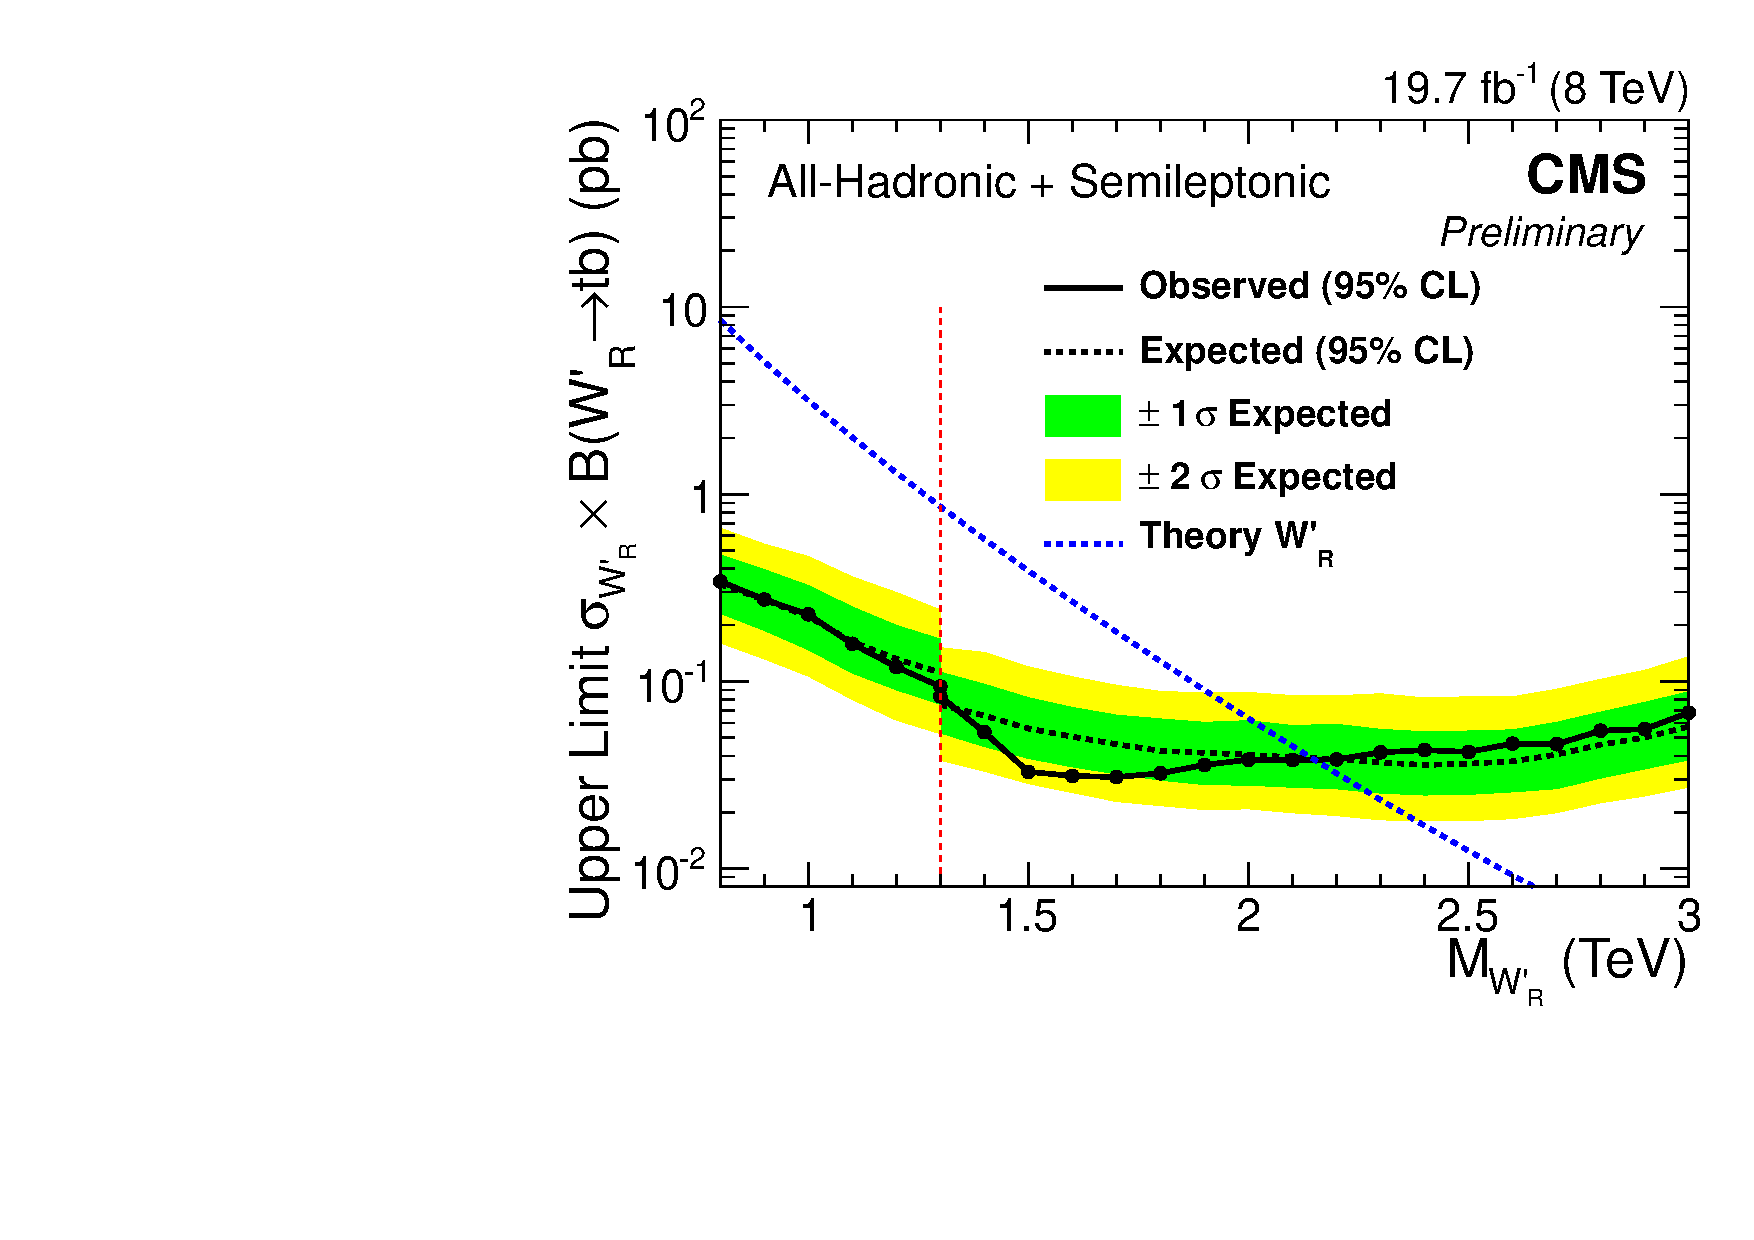
\includegraphics[width=1.0\textwidth]{AN-13-004/figs/limits_theta_Leptonic_Hadroniccomb_log.pdf}
\caption{The $\wpr_{R}$ boson 95\% C.L. production cross-section limits for the combined semileptonic and all-hadronic channels.  The expected (solid-black) and observed (dashed-black) limits as well as $\wpr_{R}$ boson theoretical cross-section (dashed-blue) are plotted for comparison.  
The uncertainty in the expected limit band is shown in green ($\pm$1$\sigma$) and yellow ($\pm$2$\sigma$).  The left of the red dashed line shows limits purely from the semileptonic channel.  The right of the red dashed line shows limits using combined sensitivity from the semileptonic and all-hadronic channels. 
These limits were extracted using the Theta limit setting framework.}
\label{figs:thetalimitcombo}
\end{figure}

\begin{figure}[htcb]
\begin{center}
\subfigure{\label{figs:GC1}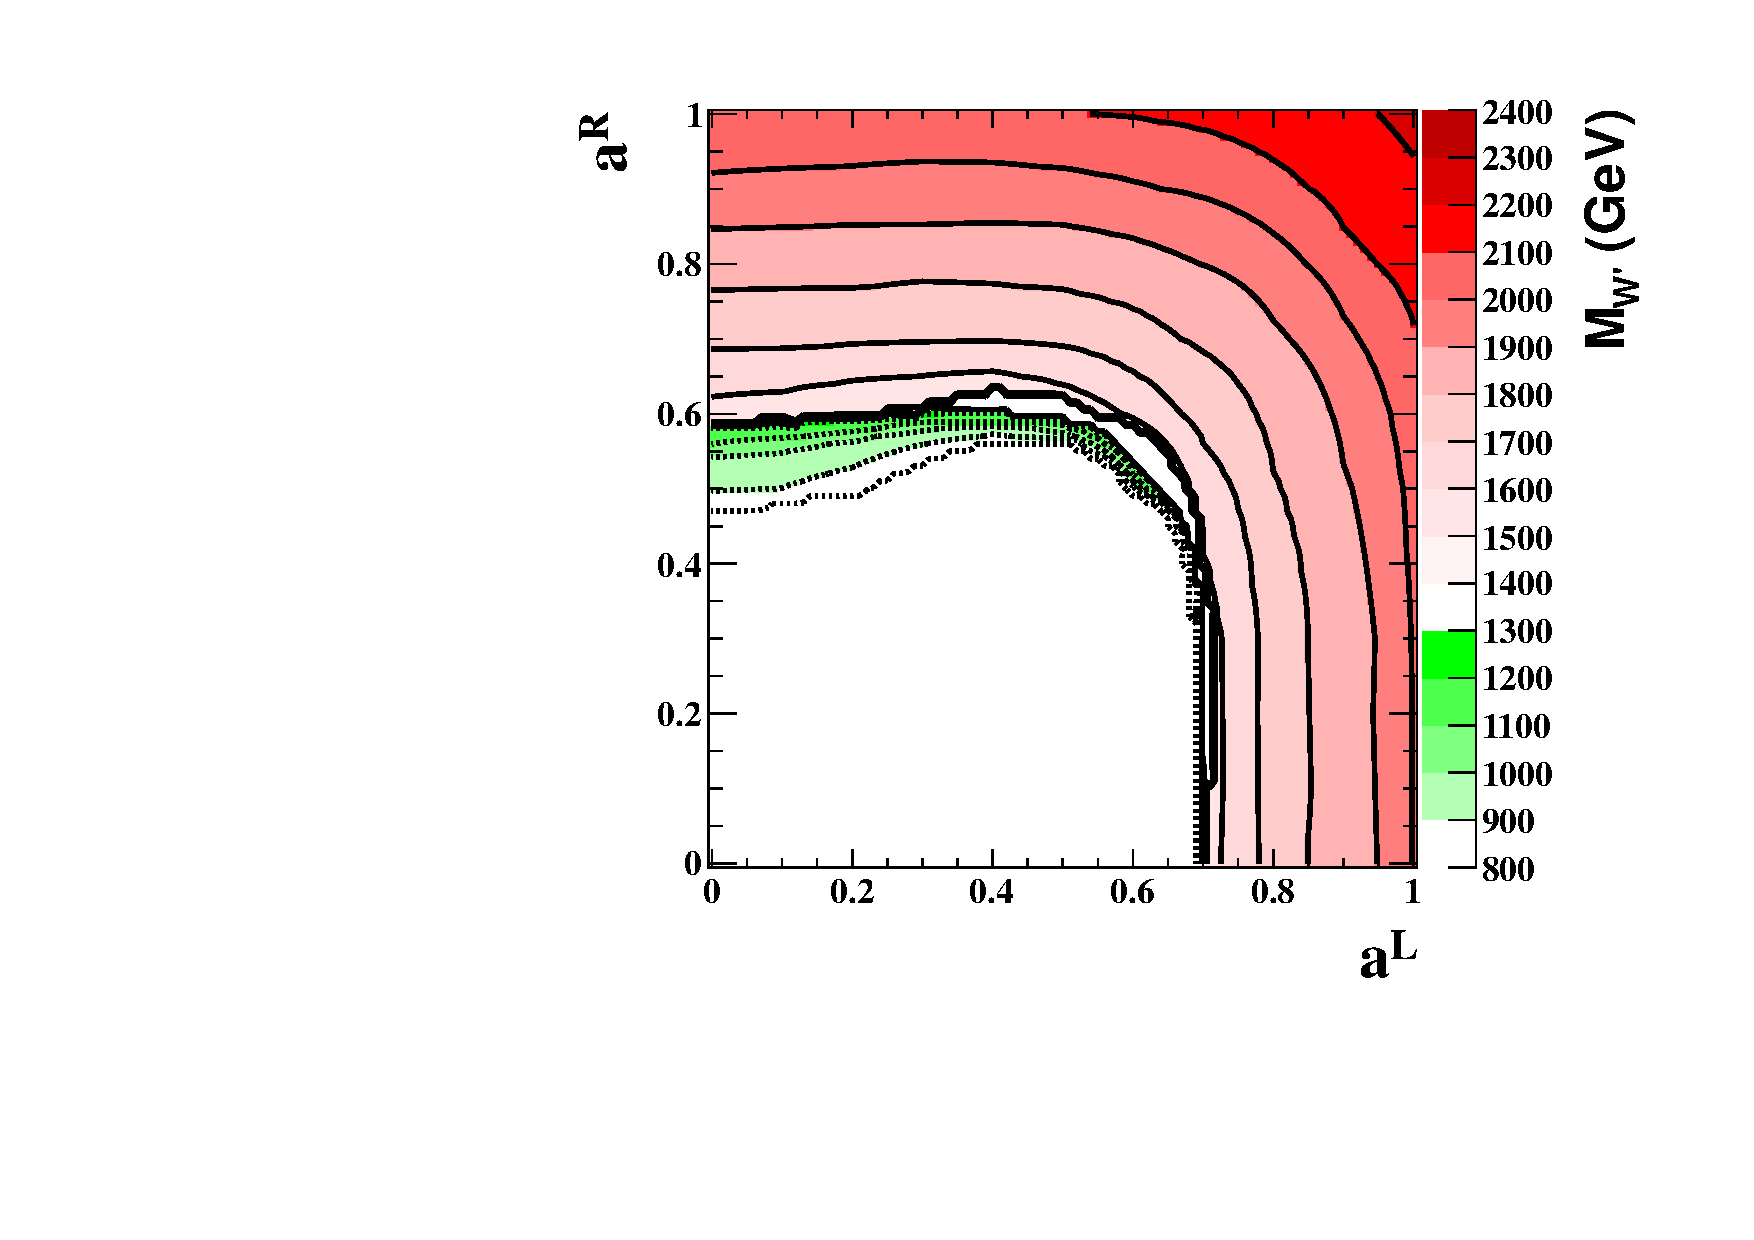
\includegraphics[width=0.7\textwidth]{AN-13-004/figs/contour_Hadronic_Leptonic_observed.pdf}}\\
\subfigure{\label{figs:GC2}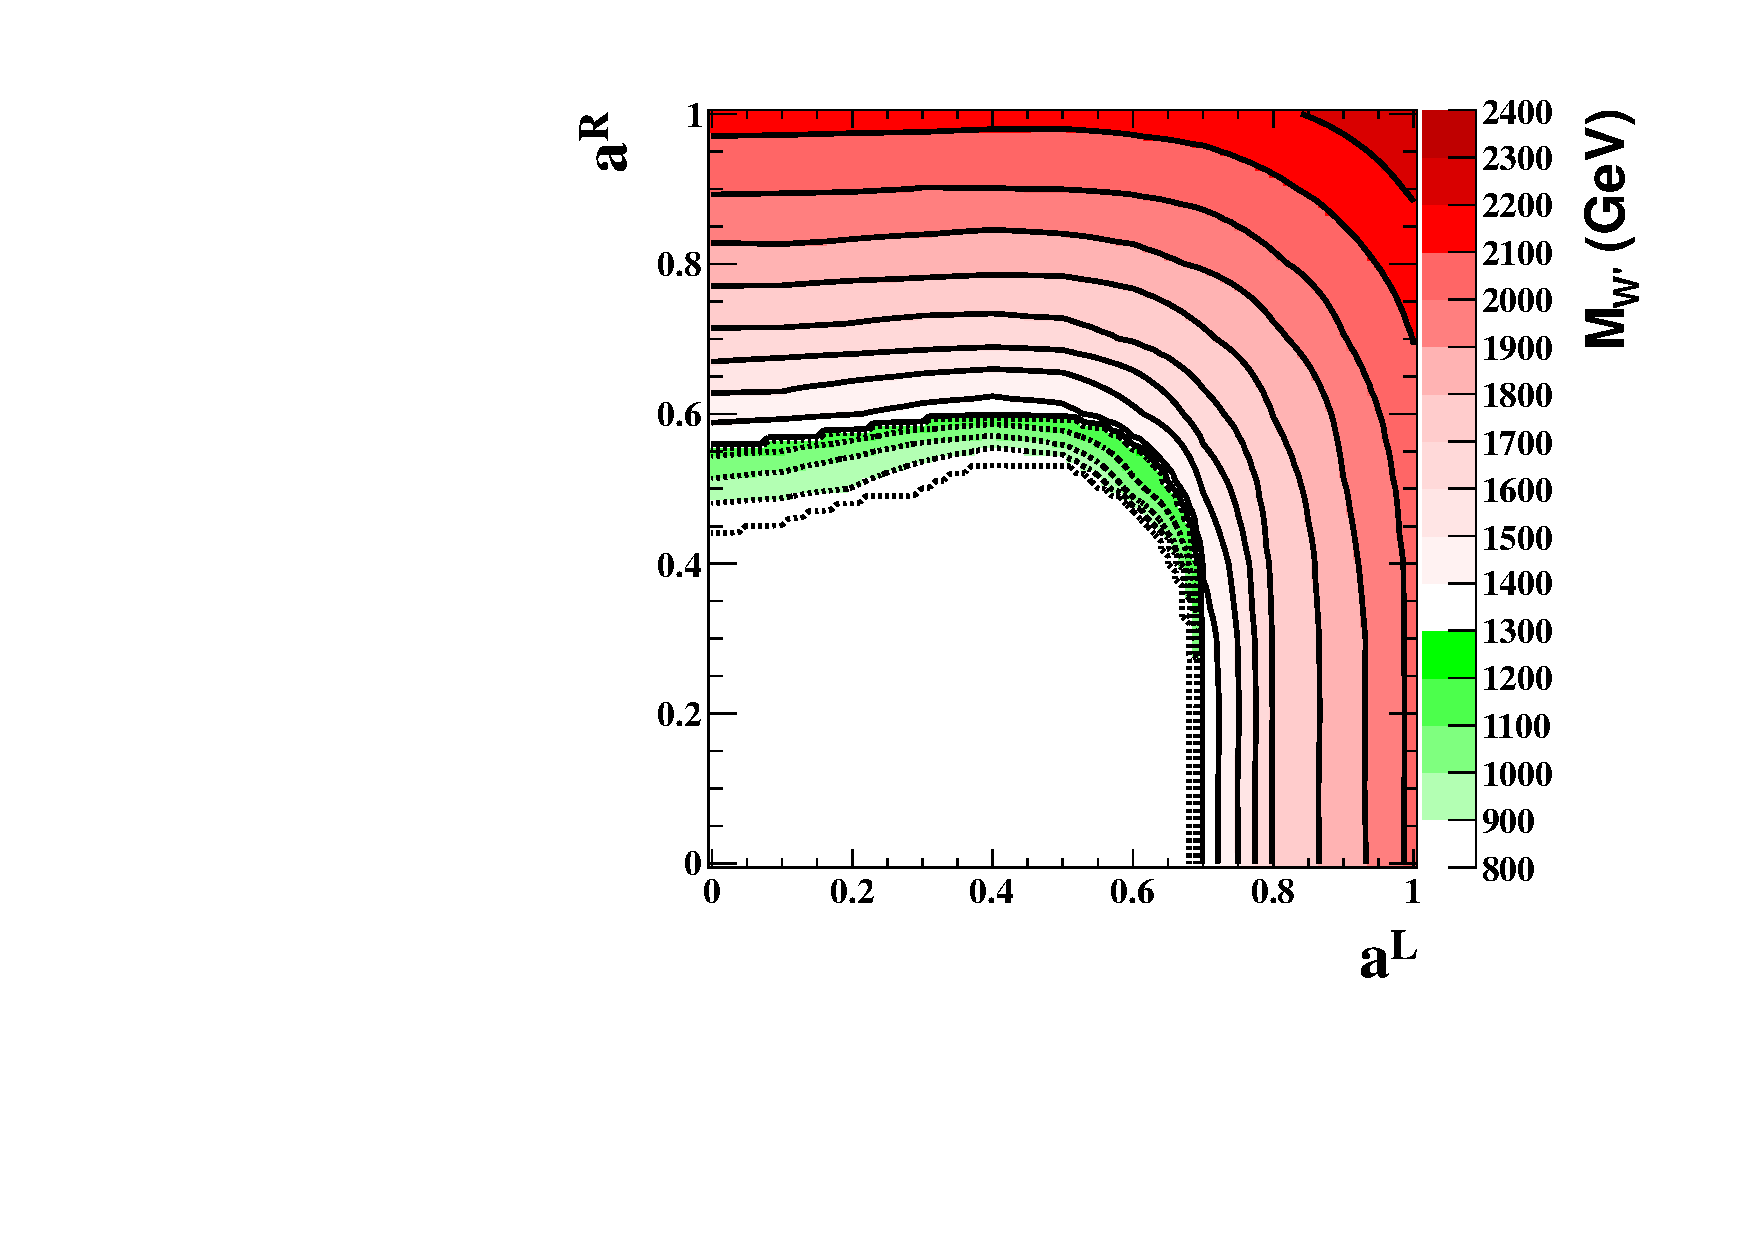
\includegraphics[width=0.7\textwidth]{AN-13-004/figs/contour_Hadronic_Leptonic_expected.pdf}}
\caption{
Plots of $M_{\wpr}$ as a function of $a^L$ and $a^R$.  The z axis colors indicate $M_{\wpr}$ where the theoretical cross section intersects the observed or expected limit band.  The red coloration indicates combined sensitivity, green indicates that the limits are purely from the semileptonic channel.  The top (bottom) plot shows observed (expected) limits.
}
\label{figs:GCLimcombo}
\end{center}
\end{figure}


\clearpage
